\documentclass[12pt,fleqn]{article}
%\documentclass[12pt,a4paper]{article}
\usepackage{natbib}
\usepackage{lineno}
%\usepackage{lscape}
%\usepackage{rotating}
%\usepackage{rotcapt, rotate}
\usepackage{amsmath,epsfig,epsf,psfrag}
\usepackage{setspace}
\usepackage{ulem}
\usepackage{xcolor}
\usepackage[labelfont=bf,labelsep=period]{caption} %for making figure and table numbers bold
\usepackage[colorlinks,bookmarksopen,bookmarksnumbered,citecolor=red,urlcolor=red]{hyperref}
\hypersetup{pdfpagemode=UseNone}

%\usepackage{a4wide,amsmath,epsfig,epsf,psfrag}


\def\be{{\ensuremath\mathbf{e}}}
\def\bx{{\ensuremath\mathbf{x}}}
\def\bX{{\ensuremath\mathbf{X}}}
\def\bthet{{\ensuremath\boldsymbol{\theta}}}
\newcommand{\VS}{V\&S}
\newcommand{\tr}{\mbox{tr}}
%\renewcommand{\refname}{\hspace{2.3in} \normalfont \normalsize LITERATURE CITED}
%this tells it to put 'Literature Cited' instead of 'References'
\bibpunct{(}{)}{,}{a}{}{;}
\oddsidemargin 0.0in
\evensidemargin 0.0in
\textwidth 6.5in
\headheight 0.0in
\topmargin 0.0in
\textheight=9.0in
%\renewcommand{\tablename}{\textbf{Table}}
%\renewcommand{\figurename}{\textbf{Figure}}
\renewcommand{\em}{\it}
\renewcommand\thefigure{B\arabic{figure}}
\renewcommand\thetable{B\arabic{table}}
\renewcommand\theequation{B.\arabic{equation}}

\begin{document}

\begin{center} \bf {\large Avoiding extrapolation bias when using statistical models to make ecological prediction}

\vspace{0.7cm}
Paul B. Conn$^{1*}$, Devin S. Johnson$^1$, and Peter L. Boveng$^1$
\end{center}
\vspace{0.5cm}

\rm
\small

\it $^1$National Marine Mammal Laboratory, Alaska Fisheries Science Center,
NOAA National Marine Fisheries Service,
Seattle, Washington 98115 U.S.A.\\

\rm \begin{flushleft}

\raggedbottom
\vspace{.5in}

\begin{center}
Appendix B: Full details of simulation study examining predictive extrapolation
\bigskip
\end{center}
\vspace{.3in}

\doublespacing

We employed a simulation study to examine the ability of the generalized independent variable hull (gIVH) to diagnose potential areas across the landscape where extrapolations from statistical species distribution models may be problematic.  Each simulation consisted of several steps, including
\begin{enumerate}
  \item Simulate four hypothetical environmental covariates over a 30 by 30 grid,
  \item Simulate animal abundance across the landscape as a function of covariates,
  \item Simulate the position of animal count quadrats across the landscape (i.e. locations where sampling is to occur) and animal counts on each quadrat,
  \item Estimate animal abundance as a function of environmental covariates according to each of three different models: a generalized linear model (GLM), a generalized additive model (GAM), and a spatio-temporal regression model (STRM).  For the latter, only a spatial dimension was considered.  All such models were specified hierarchically, with MCMC used for posterior simulation.
  \item Calculation of the gIVH as determined by (1) integrating over prior distributions for unknown parameters ($\text{gIVH}_{int}$), or (2) using realized posterior variance (i.e. after data were collected and analyzed; $\text{gIVH}_{post}$).
\end{enumerate}
We now describe each of these tasks and results of the simulation study in further detail.  All analyses were performed in the R programming environment \citep{RTeam2012}; requisite code to recreate analyses is available in the supplement.

\underline{1. Simulating environmental covariates} \\
For each simulation, we generated environmental covariates by discretizing the realizations of a Matern Cluster Process (Fig. \ref{fig:Matern}) using the rMatClust function within the R \texttt{spatstat} package \citep{BaddeleyTurner2005}.  The Matern Cluster Process is a point process that includes a total of $\kappa$ cluster centers.  Within a radius $r$ for each cluster center, a total of $n$ points are randomly distributed, where $n \sim \text{Poisson}(\lambda)$ (e.g. Fig. \ref{fig:Matern}).  For each simulated covariate, we drew $\kappa \sim U(5,10)$, $r \sim U(0.2,0.4)$, and $\lambda \sim U(200,500)$ to provide variation in the relative density and clustering for each covariate.  Next, we overlayed a 30 by 30 grid over simulated points.  To generate a hypothetical covariate, we then summed the number of points within each grid cell, and standardized so that the maximum covariate value was 1.0 (e.g. \ref{fig:Matern}).


\begin{figure}[!h]
\begin{center}
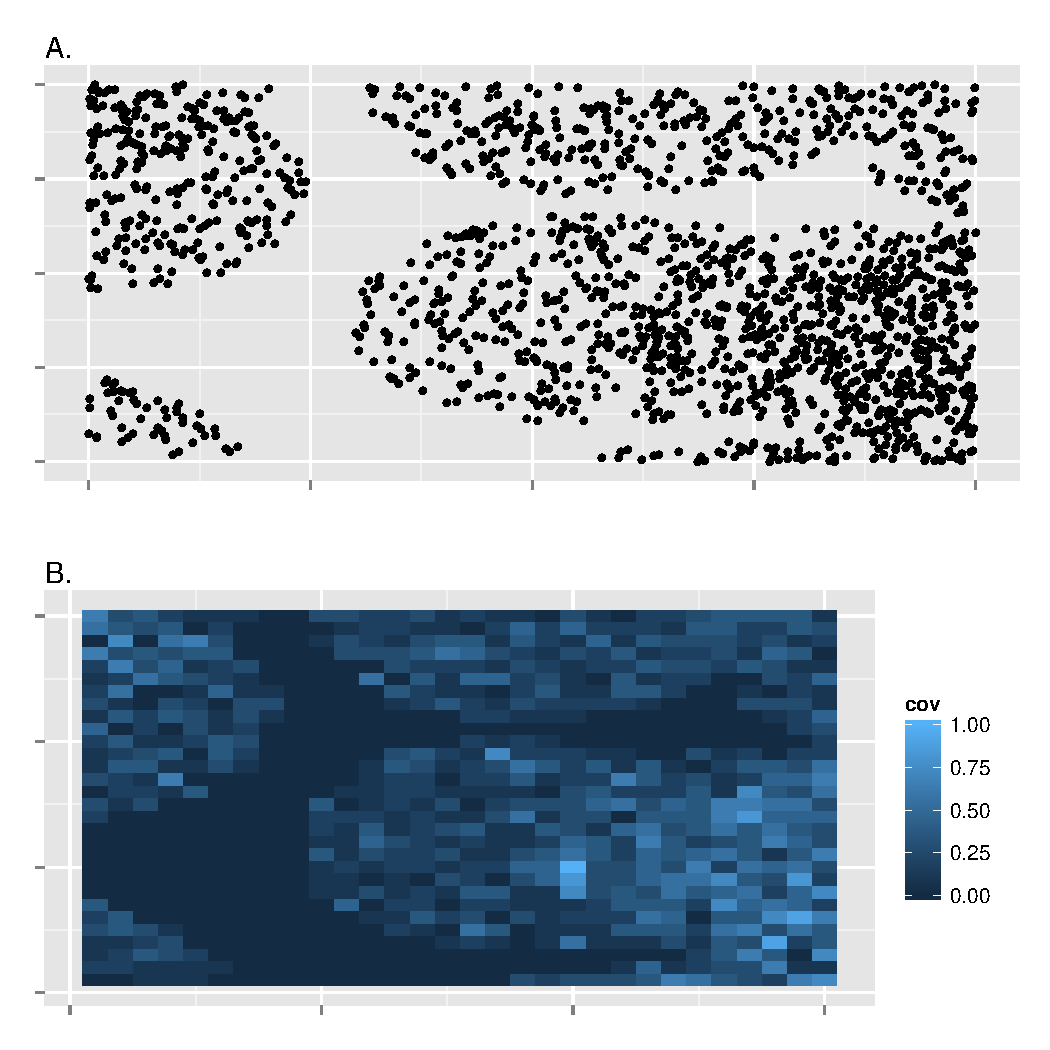
\includegraphics[width=6in]{MaternCov.pdf}
\end{center}
\caption{Environmental covariates were generated via a discretized Matern Cluster Process.  First, a Matern Cluster Process (A.) is simulated.  Next, the number of simulated points in each grid cell is counted and standardized to have a maximum of 1.0 (B.).} 
\label{fig:Matern}
\end{figure}

\underline{2. Simulating animal abundance} \\

Given values of the four simulated covariates, we generated a vector of expected log-abundance in each cell ($\boldsymbol{\mu}$) as
\begin{linenomath}
\begin{equation*}
  $\boldsymbol{\mu}$ = \beta_0 + {\bf X}\boldsymbol{\beta} + \boldsymbol{\epsilon},
\end{equation*}
\end{linenomath}
where the intercept, $\beta_0$, was drawn from a $\mathcal{N}(2.5,0.25)$ distribution, the other regression coefficients ($\boldsymbol{\beta}$) were each drawn from a $\mathcal{N}(0,0.8)$ distribution, and residual Gaussian errors ($\boldsymbol{\epsilon}$) were drawn from a $\mathcal{N}(0,0.1)$ distribution.  The design matrix ${\bf X}$ was constructed assuming linear and quadratic effects for each covariate, together with all one-way interactions for a total of 14 regression coefficients in addition to the intercept.
Next, abundance in each cell $i$ was generated as  
\begin{linenomath}
\begin{equation*}
  N_i \sim \text{Poisson}(\exp(\mu_i)).
\end{equation*}
\end{linenomath}

\underline{3. Simulating sample locations and count data} \\

For each simulated landscape, we selected 60 grid cells at random (without replacement) for sampling.  We configured simulations such that sample quadrats covered 10\% of the target grid cell, and generated animal counts for each quadrat as
\begin{linenomath}
\begin{equation*}
  C_i \sim \text{Binomial}(N_i,0.1).
\end{equation*}
\end{linenomath}

\underline{4. Estimating animal abundance} \\

For each set of count data, we attempted to estimate animal abundance over the landscape using three different hierarchical models.  The models were built to resemble a GLM, a GAM, and an STRM.




\renewcommand{\refname}{Literature Cited}
\bibliographystyle{ecology}

\bibliography{master_bib}

\end{flushleft}
\end{document}





